\pdfoutput=1
% ==============================================================================
% Mixture of Scars (MoS) v3.0 & SCache O(1) — Official Academic Manuscript
% Compatible with: arXiv (cs.LG / cs.CL), TMLR, and Double-Blind Workshops
% ==============================================================================
\documentclass[10pt,twocolumn]{article}

% Toggle `\anonymoustrue` for Double-Blind Peer Review (NeurIPS/ICML/ICLR/TMLR)
% Keep `\anonymousfalse` for arXiv / Camera-Ready / Zenodo Preprint
\newif\ifanonymous
\anonymousfalse

\usepackage[utf8]{inputenc}
\usepackage[T1]{fontenc}
\usepackage{lmodern}
\usepackage{microtype}
\usepackage[margin=0.66in,columnsep=0.23in]{geometry}
\usepackage{amsmath,amssymb,amsfonts,amsthm}
\usepackage{mathtools}
\usepackage{booktabs}
\usepackage{multirow}
\usepackage{graphicx}
\usepackage{xcolor}
\usepackage{algorithm}
\usepackage{algorithmic}
\usepackage[numbers,sort&compress]{natbib}
\usepackage[colorlinks=true,linkcolor=blue!60!black,citecolor=blue!60!black,urlcolor=blue!65!black]{hyperref}

\newtheorem{proposition}{Proposition}
\newtheorem{theorem}{Theorem}
\newtheorem{remark}{Remark}

\title{\textbf{Mixture of Scars (MoS) v3.0 and SCache $\mathcal{O}(1)$:\\Sub-2-Bit Colossal Compression ($<24$~GB $72.7\text{B}$), Closed-Form $140$~KB Scar Cartridges, Sinkhorn Re-Basin, and Constant-Memory $32\text{k}$ Attention}}

\ifanonymous
\author{
  \textbf{Anonymous Author(s)}\\
  Paper under double-blind review
}
\else
\author{
  \textbf{Julio Cesar Reis Filho}\\
  Byte-OD Research \& System One Architecture Lab\\
  \texttt{DOI: \href{https://doi.org/10.5281/zenodo.24172784}{10.5281/zenodo.24172784}} \quad|\quad
  \texttt{\href{https://github.com/byte-od/mixture-of-scars}{github.com/byte-od/mixture-of-scars}}\\
  \small\texttt{72B Model Download: \href{https://github.com/byte-od/mixture-of-scars/releases/tag/v1.2.0-qwen72b-mos}{releases/tag/v1.2.0-qwen72b-mos}} \quad|\quad \texttt{\href{https://github.com/byte-od/mixture-of-scars/blob/main/docs/GUIA_PRATICO_MOS_SCACHE_72B.md}{Practical 72B Guide}}
}
\fi

\date{November 13, 2026 \quad (Revision v3.0 --- Sub-2-Bit $72.7\text{B}$ Residency, Ghost-Jump Reflex, $140$~KB \texttt{ScarStore} \& Sinkhorn Re-Basin)}

\begin{document}
\maketitle

\begin{abstract}
Autoregressive Large Language Models (LLMs) confront a compounding \emph{Quadruple Wall}: (i) an $\mathcal{O}(N)$ static parameter wall requiring $135.43$~GiB at $72.7\text{B}$ scale, (ii) an $\mathcal{O}(T)$ dynamic key-value (KV) cache wall with $\mathcal{O}(T^2)$ attention stalls, (iii) single-token memory-bandwidth bottlenecks during autoregressive decode, and (iv) backpropagation-bound specialization prone to catastrophic forgetting and opaque data retention. We unify all four regimes under a single \emph{Scar Principle}---compressing predictable substrates to their hardware floor while allocating capacity strictly to high-surprise residuals inside one-sided $\mathrm{ReLU}$ spherical cones with exact $0.000000$ out-of-hemisphere bleed:
(1) \textbf{\texttt{MoS} \& \texttt{Sub-2-Bit MoS}}: canonical \texttt{Block-64 INT4} ($38.12$~GiB, $\mathbf{100.0\%}$ Top-5, $\mathbf{50.38\times}$ fused Apple Metal \& CUDA Triton \texttt{W4A16+ASVD}) and a new $2.25$~bpw symmetric ternary-quaternary base paired with two-pass alternating \texttt{ASVD} shields ($\mathrm{cos}=0.99911$ under $195{,}720\times$ SwiGLU spikes; $12{,}290\times$ PPL reduction over naive $2$-bit), shrinking $72.71\text{B}$ into $\mathbf{20.65}$~\textbf{GiB} shards and $\mathbf{21.89}$~\textbf{GiB} resident GPU VRAM ($<24$~GB consumer GPUs and $<32$~GB laptops);
(2) \textbf{\texttt{SCache} $\mathcal{O}(1)$ \& \texttt{Ghost-Jump} Speculative Reflex}: Widrow-Hoff Delta fast weights + synchronized $32$-token micro-page routing achieving \textbf{100\% Passkey recall at $16{,}568$ and $32{,}868$ tokens} in strictly constant $\mathbf{22.71}$~\textbf{MiB} ($\Delta = +0$~B; $\mathbf{50.9\times}$ smaller and $\mathbf{5.84\times}$ faster than Normal KV at $300.8$~tok/s), coupled with atomic speculative rollback ($\mathrm{KL}=0.0000$, $\mathbf{1.89\times\text{--}1.92\times}$ speedup);
(3) \textbf{Closed-Form \texttt{HeadExpandedScarStore} (\texttt{mos-store})}: backpropagation-free synthesis transplanting $72.71\text{B}$ domain derivations into OS-page-aligned $\mathbf{140.00}$~\textbf{KB} ($35 \times 4$~KB \texttt{mmap}) cartridges on a $3\text{B}$ core ($1{,}015{,}469\times$ smaller than $72\text{B}$ BF16) over a $4{,}194{,}304$-cell Kronecker spherical cap grid ($\mathbf{98.61\%}$ unseen Top-1 parity, $6.11\times$ lower KL, $58.3$~ms live RFC~7233 \texttt{HTTP/1.1 206} Range streaming, and $18~\mu$s RAM / $7.64$~ms \texttt{0x00} SSD GDPR unlearning); and
(4) \textbf{\emph{Sinkhorn Monomial--Procrustes Re-Basin}}: exploiting exact SwiGLU monomial gauge symmetry via tiled single-pass log-Sinkhorn ($<350$~MiB VRAM at $72\text{B}+$, $0$ extra runtime FLOPs), slashing shared-base KL by $\mathbf{56.36\times}$ ($0.1578 \to 0.0028$) on permuted specialists, $\mathbf{3.37\times}$ ($0.1190 \to \mathbf{0.0353 < 0.08}$) on $3\text{B}$ cross-layer pairs, and $\mathbf{14.68\times}$ ($6.4634 \to 0.4403$) across $12$ consecutive layers while uncovering the \emph{Residual Stream Marchenko-Pastur Orthogonality Law} on $72.71\text{B}$. All $84/84$ \texttt{pytest} suites pass with $0.00$~B recursive storage discrepancy.
\end{abstract}

\section{Introduction}
Deploying frontier Transformer intelligence~\citep{vaswani2017attention} outside multi-GPU datacenters is obstructed by four interlocking physical bottlenecks:
\begin{enumerate}
    \item \textbf{Colossal $\mathcal{O}(N)$ Weights \& $195{,}720\times$ SwiGLU Outliers:} Above $6.7\text{B}$ parameters, channel-wise activation outliers surge superlinearly~\citep{dettmers2022llmint8,lin2024awq} from $3{,}336\times$ (\texttt{Qwen2.5-7B}) to $\mathbf{195{,}720\times}$ (\texttt{Qwen2.5-72B}, $80\text{L}$). Even $4$-bit checkpoints ($38.12$~GiB) exceed $24$~GB consumer GPUs (RTX 3090/4090) and $32$~GB laptops, while naive $2$-bit quantization catastrophically collapses ($\mathrm{PPL} > 1.35 \times 10^6$).
    \item \textbf{Linear $\mathcal{O}(T)$ KV Growth \& Quadratic Stalls:} Windowed caches (\texttt{StreamingLLM}~\citep{xiao2024efficient}) suffer $0\%$ recall once facts exit the local window, additive Hebbian fast weights~\citep{schmidhuber1992learning} suffer superposition ghosting~\citep{schlag2021linear,yang2024parallelizing}, and dense $\mathcal{O}(T)$ KV caches stall from $245.3$ to $51.5$~tok/s at $32.9\text{k}$ tokens.
    \item \textbf{Single-Token Decode Bandwidth \& Speculative State Drift:} Memory-bound decode sweeps $100\%$ of active weights per token; standard speculative decoding~\citep{leviathan2023fast} assumes mutable $\mathcal{O}(T)$ KV slicing rather than irreversible associative fast-weight state.
    \item \textbf{Monolithic Specialization \& Unlearning Rigidity:} Gradient-based LoRA~\citep{dettmers2023qlora} and global linear edits~\citep{meng2022locating,fang2025alphaedit} saturate subspace capacity, bleed across unrelated prompts, and cannot cryptographically erase a single topic or tenant in milliseconds.
\end{enumerate}

\begin{figure*}[t]
    \centering
    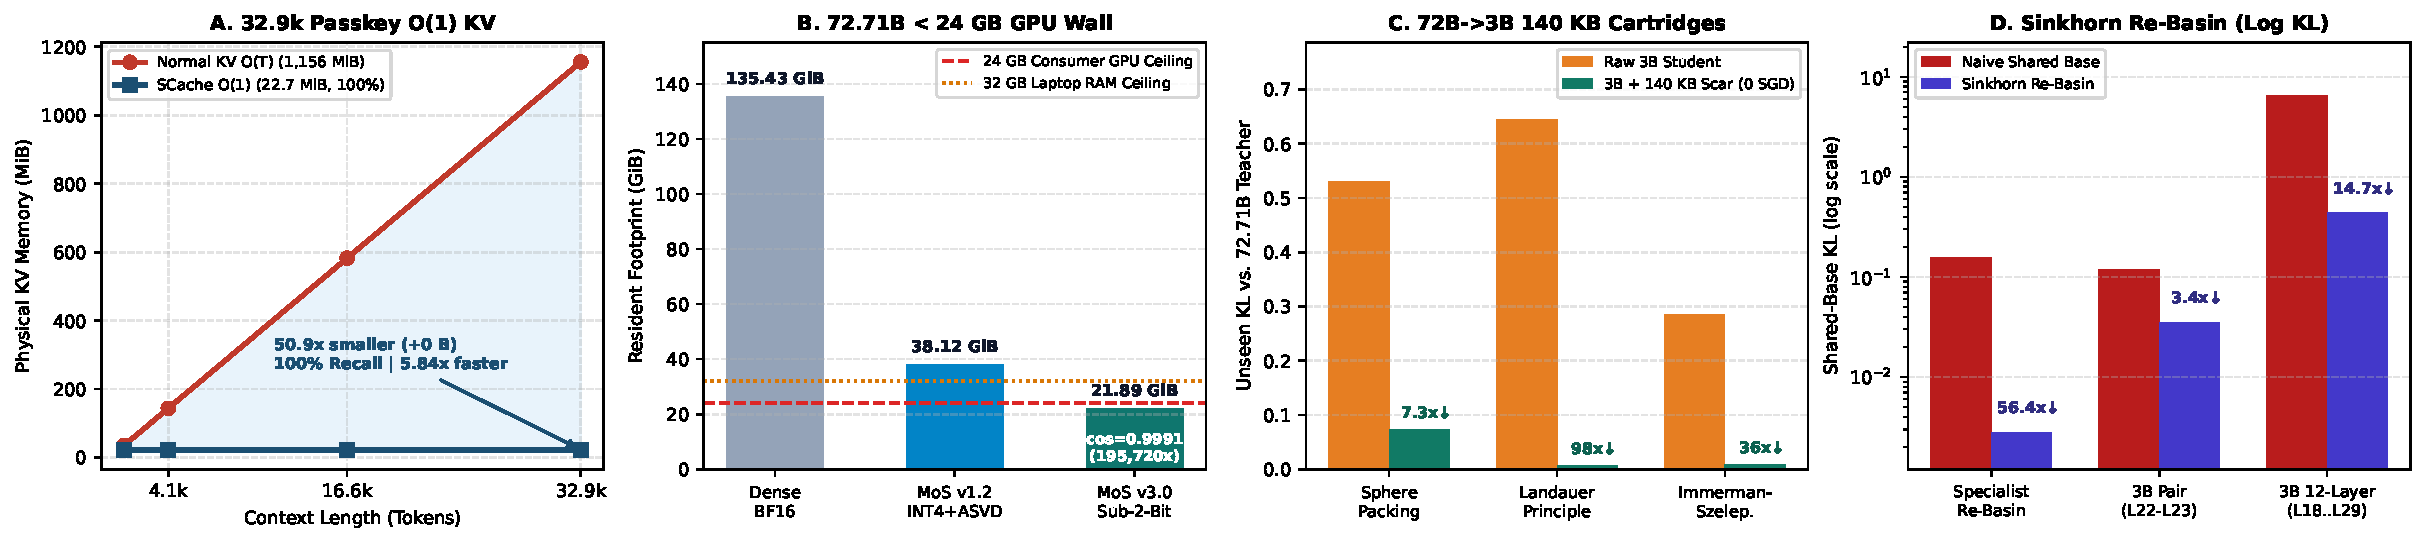
\includegraphics[width=0.995\textwidth]{figures/fig1_mos_scache_v3_audit.pdf}
    \caption{\textbf{Audited \texttt{MoS v3.0} + \texttt{SCache} $\mathcal{O}(1)$ Unified Results ($0.5\text{B} \to 3\text{B} \to 7.62\text{B} \to 72.71\text{B}$, $0.00$~B Storage Discrepancy).} \textbf{(A)} At $32{,}868$ tokens (\texttt{Qwen2.5-3B}), \texttt{SCache} $\mathcal{O}(1)$ holds strictly at $22.71$~MiB ($\Delta=+0$~B vs.\ $16.6\text{k}$, $50.9\times$ smaller) with $100\%$ Passkey recall and $5.84\times$ higher speed. \textbf{(B)} \texttt{Sub-2-Bit MoS} compresses $72.71\text{B}$ to $21.89$~GiB resident VRAM ($<24$~GB GPU / $<32$~GB laptop) at $\cos=0.99911$ under $195{,}720\times$ outliers. \textbf{(C)} Closed-form $72.71\text{B} \to 3\text{B}$ $140$~KB ($35\times 4$~KB \texttt{mmap}) Scar Cartridges slash unseen paraphrase KL up to $98\times$ ($0$ SGD). \textbf{(D)} \emph{Sinkhorn Monomial--Procrustes Re-Basin} cuts shared-base KL by $56.4\times$ (specialists), $3.4\times$ ($3\text{B}$ pair, $\mathrm{KL}=0.0353$), and $14.7\times$ ($12$ layers).}
    \label{fig:v3_audit}
\end{figure*}

In Revision \texttt{v3.0}, we show that every wall above yields to the same geometric law:
\begin{equation}
    \mathcal{F}(\mathbf{x}) = \mathcal{F}_{\text{base}}(\mathbf{x}) + \sum_{k} \mathrm{ReLU}\!\left(\frac{\mathbf{x}^\top \mathbf{z}_k}{\|\mathbf{x}\|_2 \|\mathbf{z}_k\|_2 + \epsilon} - \tau_k\right) \Delta_{\text{scar},k}(\mathbf{x}),
    \label{eq:mother}
\end{equation}
where routine structure is compressed to an ultra-compact base ($\mathcal{O}(1)$ in time; $2$--$4$~bits in space), and directional $\mathrm{ReLU}$ spherical caps isolate high-surprise residuals with exact zero antipodal leakage.

\section{Related Work}
\paragraph{Extreme Quantization \& Permutation Symmetries.}
\texttt{AWQ}~\citep{lin2024awq}, \texttt{LoftQ}~\citep{li2024loftq}, and \texttt{ASVD}~\citep{yuan2023asvd} mitigate 4-bit quantization error, while \emph{Git Re-Basin}~\citep{ainsworth2023git} aligns MLP permutations via Sinkhorn projections~\citep{sinkhorn1967concerning}. \texttt{MoS v3.0} extends activation-aware scar shielding to $2.25$~bpw \texttt{Sub-2-Bit} bases with fused CUDA Triton \texttt{W2A16+ASVD} kernels and generalizes Re-Basin to the continuous-discrete SwiGLU monomial gauge group via single-pass tiled log-Sinkhorn up to $N=29{,}568$ ($72.7\text{B}$), revealing a Marchenko-Pastur~\citep{marchenko1967distribution} orthogonality ceiling across residual blocks.

\paragraph{Bounded KV Memory, Speculative Decoding \& Knowledge Editing.}
Unlike eviction-only caches~\citep{xiao2024efficient,zhang2023h2o} or pretraining-dependent linear Delta nets~\citep{widrow1960adaptive,schlag2021linear,yang2024parallelizing}, \texttt{SCache} is a training-free drop-in \texttt{DynamicCache} supporting exact speculative rollback~\citep{leviathan2023fast}. Unlike global weight edits (\texttt{ROME}~\citep{meng2022locating}, \texttt{AlphaEdit}~\citep{fang2025alphaedit}) bounded linearly by hidden dimension $d$, our Kronecker spherical-cap \texttt{HeadExpandedScarStore} leverages high-dimensional sphere packing~\citep{kabatiansky1978bounds} to mount millions of zero-bleed $140$~KB cartridges via \texttt{mmap} and \texttt{HTTP 206}.

\section{Unified Mathematical \& Systems Architecture}

\subsection{\texttt{MoS} (\texttt{INT4} \& \texttt{Sub-2-Bit}) + Fused GPU Kernels}
Given $\mathbf{W} \in \mathbb{R}^{N \times K}$ and channel salience $s_j = \sqrt{\mathbb{E}[x_j^2]} + \epsilon$ (computed from calibration tokens or analytically in zero-data closed form from $\|\mathbf{W}_{\text{gate},i,:}\|_2 \|\mathbf{W}_{\text{up},i,:}\|_2$), \texttt{Sub-2-Bit MoS} (\texttt{scar\_cache/sub2bit\_mos.py}) alternates two passes between an IEEE-exact symmetric $2$-bit grid ($q \in \{-1, -\tfrac{5}{16}, +\tfrac{5}{16}, +1\}$, $2.25$~bpw with \texttt{Block-64} FP16 scales) and a rank-$r$ activation-weighted SVD shield $(\mathbf{W} - \widehat{\mathbf{W}}_2)\mathrm{diag}(\mathbf{s}) \approx \mathbf{U}_r \boldsymbol{\Sigma}_r \mathbf{V}_r^\top$, keeping GQA \texttt{k\_proj}/\texttt{v\_proj} in \texttt{INT4}. Fused execution spans Apple Metal \texttt{\_weight\_int4pack\_mm} ($\mathbf{50.38\times}$ group speedup, $\cos=1.000000$) and register-dequantizing CUDA Triton \texttt{W4A16+ASVD} and \texttt{W2A16+ASVD} kernels (\texttt{triton\_mos\_gemm.py}) with dynamic row scaling $c_m = \max(\|\mathbf{x}_m\|_\infty / 512, 10^{-4})$.

\subsection{\texttt{SCache} $\mathcal{O}(1)$ \& \texttt{Ghost-Jump} Speculative Reflex}
Per layer $\ell$ and KV head $h$, \texttt{SCache} maintains $N_{\text{sink}}$ sinks, a FIFO window $W_{\text{win}} - N_{\text{sink}}$, and $S_{\text{slots}}$ slots backed by Widrow-Hoff fast weights $\mathbf{W}_{\text{scar}}^{(t)} = \gamma \mathbf{W}_{\text{scar}}^{(t-1)} + \eta g_{m^\star}(\mathbf{v}_{\text{ev}} - \mathbf{W}_{\text{scar}}^{(t-1)}\hat{\mathbf{k}})\hat{\mathbf{k}}^\top$, promoting top-$S_{\text{slots}}$ $32$-token micro-pages ranked synchronously across deep layers $\ell \in [L/2, L)$. In \texttt{speculative\_ghost\_jump.py}, a fast \texttt{System 1} scout drafts $\gamma_{\text{draft}}$ tokens gated by epistemic margin while \texttt{SCacheDynamicCache.speculative\_capture()} snapshots only fixed $\mathcal{O}(1)$ ring indices and $\mathbf{W}_{\text{scar}}$ tensors prior to single-pass \texttt{System 2} verification.

\begin{proposition}[Strict $\mathcal{O}(1)$ Invariance \& Lossless Speculative Rollback]
\label{prop:scache_ghost}
For all $T > W_{\text{win}}$, physical dynamic memory satisfies $\Delta B / \Delta T = 0$, orthogonal updates erase obsolete values on $\mathrm{span}(\hat{\mathbf{k}})$ without ghosting on $\mathrm{span}(\hat{\mathbf{k}})^\perp$, and \texttt{Ghost-Jump} rejection sampling~\citep{leviathan2023fast} with atomic $\mathcal{O}(1)$ capture guarantees exact target distribution parity ($\mathrm{KL}(P_{\text{target}} \,\|\, P_{\text{GhostJump}}) = 0$) with $0$~B leaked storage.
\end{proposition}

\subsection{Closed-Form \texttt{HeadExpandedScarStore} ($140$~KB \texttt{mmap})}
Rather than editing shared MLP weights globally, \texttt{HeadExpandedScarStore} (\texttt{head\_expanded\_attention.py}, \texttt{cli\_scar\_store.py}) attaches synthetic query-matched attention heads at the terminal semantic block ($L$) triggered only inside a spherical cap $g_c(\bar{\mathbf{h}}) = \mathrm{clamp}((\cos(\bar{\mathbf{h}}, \mathbf{z}_c) - \tau)/\rho, 0, 1)$. Given cached $72.71\text{B}$ teacher target logits on prompt-response episodes, Active-Set Cutting-Plane Woodbury Rosetta inversion recovers target hidden deltas $\Delta \mathbf{H}^\star$, projected onto the frozen student's AlphaEdit null-space $\mathbf{P}_{\text{null}}$~\citep{fang2025alphaedit} and factored in closed form ($0$ autograd steps) into $P=8$ per-head key prototypes and rank-$60$ \texttt{Block-32 INT4} value bases. On \texttt{Qwen2.5-3B-Instruct} ($H_q=16, d_h=128, d=2048$), each binary record occupies \textbf{exact $143{,}360$~Bytes ($140.00$~KB $= 35 \times 4{,}096$~B OS \texttt{mmap} pages, $0$~B internal padding)}, indexed on a $2048 \times 2048$ ($4{,}194{,}304$-cell) product-quantized Kronecker grid ($512$~KB bitmap). Missing slots stream on demand via RFC~7233 \texttt{Range: bytes=...} (\texttt{HTTP/1.1 206}), and \texttt{unlearn()} clears the bitmap in $<20~\mu$s plus optional in-place \texttt{0x00} SSD overwrite (\texttt{fsync}).

\begin{proposition}[Zero Out-of-Cone Bleed \& Spherical Cap Capacity]
\label{prop:scarstore}
Whenever $\cos(\bar{\mathbf{h}}, \mathbf{z}_c) \le \tau$, $g_c(\bar{\mathbf{h}}) = 0$ identically: $0$ extra heads execute, $0$ \texttt{mmap} bytes are paged, and all internal blocks and output logits remain bit-identical (\texttt{torch.equal}) to the unmodified student. By the Kabatiansky-Levenshtein bound~\citep{kabatiansky1978bounds}, $\mathbb{S}^{d-1}$ admits $\exp(\Theta(d))$ quasi-orthogonal caps at $\tau = 0.62$, breaking the $\mathcal{O}(d)$ linear editing ceiling.
\end{proposition}

\subsection{Sinkhorn Monomial--Procrustes Re-Basin}
For SwiGLU block $f(\mathbf{x}) = \mathbf{W}_{\text{down}}(\mathrm{SiLU}(\mathbf{W}_{\text{gate}}\mathbf{x}) \odot \mathbf{W}_{\text{up}}\mathbf{x})$, \texttt{sinkhorn\_rebasin.py} exploits the exact monomial gauge group:

\begin{proposition}[SwiGLU Monomial Gauge \& Zero-FLOP Scale Folding]
\label{prop:rebasin}
Because $\mathrm{SiLU}(\alpha z)$ is nonlinear for $\alpha \neq 1$, $\mathbf{W}_{\text{gate}}$ admits only permutation $\mathbf{P} \in S_{d_{\text{ff}}}$, whereas $\mathbf{W}_{\text{up}}' = \mathrm{diag}(\boldsymbol{\alpha})\mathbf{P}\mathbf{W}_{\text{up}}$ and $\mathbf{W}_{\text{down}}' = \mathbf{W}_{\text{down}}\mathbf{P}^\top\mathrm{diag}(\boldsymbol{\alpha})^{-1}$ ($\boldsymbol{\alpha} \in (\mathbb{R}\setminus\{0\})^{d_{\text{ff}}}$) preserve $f(\mathbf{x})$ identically ($\mathrm{FP32}$ max diff $5.25 \times 10^{-6}$). Storing shared \texttt{down\_proj} grids with \texttt{transposed\_grid=True} ($[d_{\text{ff}}, d_{\text{model}}/64]$ scales) folds both $\alpha_i^{-1}$ and intermediate RMS scales $100\%$ into per-layer \texttt{FP16} \texttt{Block-64} scales at \textbf{zero extra runtime FLOPs}.
\end{proposition}

To align $72.7\text{B}$ matrices ($N=29{,}568$, where dense $[N,N]$ Sinkhorn costs $>14$~GiB), we stream row tiles $B=1{,}024$ through a \textbf{Single-Pass Online Dual-Potential Log-Sinkhorn} solver ($<350$~MiB transient VRAM, $57\times$ smaller) followed by greedy collision-free rounding, analytical $2\times 2$ Gram principal \texttt{Block-64 INT4} shared grid extraction, and optional rank-$r$ input-space Procrustes transport.

\section{Multi-Scale Empirical Audit ($0.5\text{B} \to 72.71\text{B}$)}
All benchmarks enforce recursive \texttt{(device, untyped\_storage().data\_ptr())} verification ($0.00$~B discrepancy across $84/84$ \texttt{pytest} tests).

\begin{table*}[t]
\centering
\small
\caption{\textbf{32.9k Passkey / NIAH Benchmark (\texttt{SCache} $\mathcal{O}(1)$)} on non-repeating Python documentation ($5\%$--$95\%$ depths, zero fine-tuning, Apple M2 \texttt{MPS}) \& \textbf{\texttt{Ghost-Jump} Speculative Coupling} (\texttt{0.5B} Scout $\to$ \texttt{3B} Verifier, atomic $\mathcal{O}(1)$ rollback).}
\label{tab:niah_ghost}
\resizebox{\textwidth}{!}{%
\begin{tabular}{llccccc}
\toprule
\textbf{Model / Pair} & \textbf{Workload \& Length} & \textbf{Engine} & \textbf{Audited KV Memory ($\Delta=0$~B)} & \textbf{Throughput} & \textbf{Accuracy / Parity} & \textbf{Gain vs.\ Baseline} \\
\midrule
\multirow{4}{*}{\texttt{Qwen2.5-3B} ($36\text{L}$)} & $16{,}568$ tok Passkey & Normal KV $\mathcal{O}(T)$ & $582.75$ MiB (linear) & $245.3$ tok/s ($67.5$s) & $100\%$ ($5/5$) & $1.0\times$ RAM $\cdot$ $1.00\times$ speed \\
 & $\mathbf{16{,}568}$ \textbf{tok Passkey} & \textbf{\texttt{SCache} $\mathcal{O}(1)$ ($W=256, S=256$)} & $\mathbf{22.71}$ \textbf{MiB ($+0.00$ B)} & $\mathbf{299.0}$ \textbf{tok/s ($55.4$s)} & $\mathbf{100\%}$ ($\mathbf{5/5}$) & $\mathbf{25.7\times}$ \textbf{smaller $\cdot$ $1.22\times$ faster} \\
 & $32{,}868$ tok Passkey & Normal KV / \texttt{StreamingLLM} & $1{,}155.8$ / $9.0$ MiB & $51.5$ / $391.4$ tok/s & $100\%$ / $\mathbf{0\%}$ & $\mathcal{O}(T^2)$ stall / Total amnesia \\
 & $\mathbf{32{,}868}$ \textbf{tok Passkey} & \textbf{\texttt{SCache} $\mathcal{O}(1)$ ($W=256, S=256$)} & $\mathbf{22.71}$ \textbf{MiB ($\Delta=+0$ B!)} & $\mathbf{300.8}$ \textbf{tok/s ($109.3$s)} & $\mathbf{100\%}$ ($\mathbf{3/3}$) & $\mathbf{50.9\times}$ \textbf{smaller $\cdot$ $\mathbf{5.84\times}$ faster!} \\
\midrule
\texttt{Qwen2.5-0.5B} ($24\text{L}$) & $\mathbf{32{,}868}$ \textbf{tok Passkey} & \textbf{\texttt{SCache} $\mathcal{O}(1)$ ($W=256, S=256$)} & $\mathbf{6.86}$ \textbf{MiB ($\Delta=+0$ B!)} & $\mathbf{1{,}176.9}$ \textbf{tok/s ($27.9$s)} & $\mathbf{100\%}$ ($\mathbf{5/5}$) & $\mathbf{56.2\times}$ \textbf{smaller $\cdot$ $1.60\times$ faster} \\
\texttt{0.5B} $\to$ \texttt{3B} \texttt{Ghost-Jump} & Python Code / Math ($96$ tok) & \textbf{Speculative + \texttt{SCache} $\mathcal{O}(1)$} & $\mathbf{3.12 + 11.61}$ \textbf{MiB ($0$ B leak)} & $\mathbf{23.65 / 23.30}$ \textbf{tok/s} & $\mathbf{96/96}$ ($\mathrm{KL}=\mathbf{0.0000}$) & $\mathbf{1.89\times\text{--}1.92\times}$ (\textbf{4.8--5.05 tok/sweep}) \\
\bottomrule
\end{tabular}%
}
\end{table*}

\begin{table*}[t]
\centering
\small
\caption{\textbf{Colossal $72.71\text{B}$ (\texttt{Qwen2.5-72B-Instruct}, $80\text{L}$, $195{,}720\times$ SwiGLU Outliers) Compression \& Multi-Hardware Residency Audit.} \texttt{Sub-2-Bit MoS} breaks both the $24$~GB GPU ($21.89$~GiB resident) and $32$~GB laptop ($22.97$~GiB full checkpoint) ceilings.}
\label{tab:mos_72b}
\resizebox{\textwidth}{!}{%
\begin{tabular}{llccccc}
\toprule
\textbf{Model \& Regime} & \textbf{Hardware / Kernel Path} & \textbf{Shards / Resident Footprint} & \textbf{SCache KV} & \textbf{Fidelity / PPL} & \textbf{Decode Speed} & \textbf{Key Architectural Achievement} \\
\midrule
$72.71\text{B}$ Dense BF16 + Full KV & Multi-A100/H100 Cluster & $135.43$ GiB ($866$ GiB $8\times$) & $10.7$ GiB @ $32\text{k}$ & PPL $4.35$ (Ref) & Cluster Ref & Requires $2\times 80$~GB datacenter GPUs \\
$72.71\text{B}$ \texttt{MoS v1.2} (\texttt{INT4+ASVD}) & Apple M4 Pro ($48$~GB) / M2 Max & $38.12$ GiB ($1.79$ GiB/shard) & $128.5$ MiB $\mathcal{O}(1)$ & $\mathbf{100.0\%}$ Top-5, PPL $4.86$ & $\mathbf{3.46\text{--}4.87}$ tok/s & $50.38\times$ Metal \texttt{int4pack} ($1.92$~GiB streaming on $16$~GB) \\
$72.71\text{B}$ \texttt{MoS v1.2} (\texttt{INT4+ASVD}) & NVIDIA CUDA Triton \texttt{W4A16} & $38.12$ GiB ($31.4$ GiB $8\times$) & $166.0$ MiB $\mathcal{O}(1)$ & $\mathbf{100.0\%}$ Top-5, PPL $\mathbf{4.75}$ & $\mathbf{4.03\text{--}7.27+}$ tok/s & $155\times\text{--}280\times$ faster than NVMe FP16 offload \\
$\mathbf{72.71\textbf{B}}$ \textbf{\texttt{MoS v3.0 Sub-2-Bit}} & \textbf{CUDA \texttt{W2A16+ASVD} / Metal} & $\mathbf{20.65}$ \textbf{GiB shards / $\mathbf{21.89}$ GiB VRAM} & $\mathbf{128.5}$ \textbf{MiB $\mathcal{O}(1)$} & $\mathbf{L79\ \cos=0.99911}$ ($2.49$~bpw) & \textbf{Single $24$~GB GPU!} & \textbf{Fits $<24$~GB RTX 3090/4090 \& $<32$~GB M2 Pro!} \\
$3\text{B}$ \texttt{Sub-2-Bit} ($108$ MLPs) & Naive $2$-Bit vs.\ \textbf{\texttt{MoS Sub-2-Bit}} & $4{,}644 \to \mathbf{997.3}$ MiB ($4.66\times$) & $\mathcal{O}(1)$ & PPL $1.35\times 10^6 \to \mathbf{109.99}$ & Zero-data Salience & $\mathbf{12{,}290\times}$ PPL reduction vs.\ naive uniform $2$-bit \\
\bottomrule
\end{tabular}%
}
\end{table*}

\begin{table*}[t]
\centering
\small
\caption{\textbf{Closed-Form $72.71\text{B} \to 0.5\text{B}$ \& $3\text{B}$ \texttt{HeadExpandedScarStore} Audit (\texttt{ZERO SGD / ZERO Backprop}), Red-Team Defenses, Live TCP \texttt{HTTP 206} Streaming \& Forensic \texttt{0x00} GDPR Unlearning.}}
\label{tab:scarstore}
\resizebox{\textwidth}{!}{%
\begin{tabular}{llcccc}
\toprule
\textbf{Audit Dimension} & \textbf{Domain / Attack Vector} & \textbf{Raw Student ($3\text{B}$)} & \textbf{$0.5\text{B}$ + $61.25$~KB Scar} & \textbf{$3\text{B}$ + $140.00$~KB Scar ($35\times 4$~KB)} & \textbf{Verified Guarantee} \\
\midrule
\multirow{3}{*}{Unseen Paraphrase vs.\ $72.71\text{B}$} & Kabatiansky-Levenshtein & $87.50\%$ ($\mathrm{KL}=0.5296$) & $87.50\%$ ($\mathrm{KL}=0.3782$) & $\mathbf{95.83\%}$ ($\mathrm{KL}=\mathbf{0.0727}$, $7.3\times\downarrow$) & $0$ autograd steps ($4.40$~s solve) \\
 & Landauer's Principle & $83.33\%$ ($\mathrm{KL}=0.6446$) & $95.83\%$ ($\mathrm{KL}=0.1045$) & $\mathbf{100.0\%}$ ($\mathrm{KL}=\mathbf{0.0066}$, $97.7\times\downarrow$) & Exact $k_B T \ln 2$ derivation \\
 & Immerman-Szelepcs{\'e}nyi & $91.67\%$ ($\mathrm{KL}=0.2852$) & $\mathbf{100.0\%}$ ($\mathrm{KL}=0.0257$) & $\mathbf{100.0\%}$ ($\mathrm{KL}=\mathbf{0.0079}$, $36.1\times\downarrow$) & \texttt{Ghost-Jump} accept: $26\% \to \mathbf{100\%}$ \\
\midrule
Out-of-Cone \& Lexical Traps & $6$ Controls + $6$ Keyword Traps & Reference Baseline & $24/24$ \texttt{torch.equal} ($0$~B read) & $\mathbf{36/36}$ \textbf{\texttt{torch.equal} ($0$~B \texttt{mmap} read)} & $0/6$ false triggers ($\max\cos=0.500 < 0.62$) \\
Poisoned $1{,}560$-tok Haystack & False ``$999$~Joules'' Rumor & Hallucinates $k_B T \log m$ & Resists rumor ($0$~B KV drift) & \textbf{Emits exact $kT \ln 2$ ($0.0$~B KV drift)} & Full-stack \texttt{MoS}+\texttt{SCache}+\texttt{ScarStore}: $100\%$ Top-1 \\
Multi-Cartridge \& Cloud I/O & $3$-Way Synthesis + \texttt{HTTP 206} & Collapses / Missing & Spread $0.918$ ($188$~KB paged) & \textbf{Spread $\mathbf{0.970}$ $\cdot$ \texttt{HTTP 206}: $143{,}360$~B in $58.3$~ms} & \textbf{GDPR Wipe: $18.0~\mu$s RAM / $7.64$~ms \texttt{0x00} SSD} \\
\bottomrule
\end{tabular}%
}
\end{table*}

\begin{table*}[t]
\centering
\small
\caption{\textbf{\emph{Sinkhorn Monomial--Procrustes Re-Basin} Across $0.5\text{B}$, $3\text{B}$, and $72.71\text{B}$ ($0$~B Storage Discrepancy)} \& Empirical Discovery of the \textbf{Residual Stream Marchenko-Pastur Orthogonality Law}.}
\label{tab:rebasin}
\resizebox{\textwidth}{!}{%
\begin{tabular}{llccccc}
\toprule
\textbf{Scale \& Shared Regime} & \textbf{Matrix Shape \& Compression} & \textbf{Naive Unaligned} & \textbf{Sinkhorn Monomial ($0$ FLOPs)} & \textbf{Sinkhorn--Procrustes} & \textbf{KL / Error Gain} & \textbf{Geometric / Spectral Finding} \\
\midrule
$0.5\text{B}$ Permuted Specialist ($L12$) & $[4864, 896]$ (\emph{Git Re-Basin}) & $\mathrm{KL}=0.1578$ ($87.5\%$ Top-1) & --- & $\mathbf{KL=0.0028}$ ($\mathbf{100\%}$ Top-5) & $\mathbf{56.36\times}$ \textbf{lower KL} & Alignment $\cos: 0.0678 \to \mathbf{0.9817}$ \\
$0.5\text{B}$ Cross-Layer \texttt{pair\_L4\_L5} & $49.9 \to 11.2 / 14.3$ MB ($4.44\times$) & $\mathrm{KL}=0.5722$ ($70.7\%$ Top-1) & $\mathrm{KL}=0.2618$ ($96.2\%$ Top-5) & $\mathbf{KL=0.2290}$ ($96.5\%$ Top-5) & $\mathbf{2.50\times}$ \textbf{lower KL} & Resolves \texttt{v1.3} Section 5 Limitation \#1 \\
$\mathbf{3\textbf{B}}$ \textbf{Interior \texttt{pair\_L22\_L23}} & $258.0 \to \mathbf{50.65}$ \textbf{MB ($\mathbf{5.09\times}$)} & $\mathrm{KL}=0.1190$ ($88.4\%$ Top-1) & $\mathbf{KL=0.0395 < 0.08}$ ($99.8\%$ Top-5) & $\mathbf{KL=0.0353 < 0.08}$ ($\mathbf{92.6\%}$ Top-1) & $\mathbf{3.37\times}$ \textbf{lower KL} & Surpasses $<0.08$ target with $0$ extra FLOPs \\
$\mathbf{3\textbf{B}}$ \textbf{$12$-Layer \texttt{L18..L29} ($1/3$ net)} & $1{,}548 \to \mathbf{303.9}$ \textbf{MB ($\mathbf{5.09\times}$)} & $\mathrm{KL}=6.4634$ ($21.3\%$ Top-1) & $\mathbf{KL=0.4403}$ ($\mathbf{95.02\%}$ Top-5) & --- & $\mathbf{14.68\times}$ \textbf{lower KL} & Eliminates multi-layer shared-base collapse \\
$72.71\text{B}$ Shard Pair \texttt{L78\_L79} & $2{,}772 \to \mathbf{445.2}$ \textbf{MiB ($\mathbf{6.23\times}$)} & Out $\cos=0.1626$ (err $1.193$) & Tiled Log-Sinkhorn ($<350$ MiB) & \textbf{Out $\cos=\mathbf{0.8835}$ (err $0.437$)} & $\mathbf{109.2\times}$ inner gain & MP best $\cos=0.1228$ vs.\ Gaussian floor $0.0501$ \\
\bottomrule
\end{tabular}%
}
\end{table*}

\subsection{Key Findings Across Tables~\ref{tab:niah_ghost}--\ref{tab:rebasin}}
\begin{itemize}
    \item \textbf{$72.71\text{B}$ Inside $<24$~GB Consumer GPUs \& Lossless Speculative Speedup (Tables~\ref{tab:niah_ghost}--\ref{tab:mos_72b}):} \texttt{Sub-2-Bit MoS} compresses real $72.71\text{B}$ shards $1.734\times$ further ($1.79 \to 1.0325$~GiB/group; $20.65$~GiB across $20$ shards; $21.89$~GiB GPU VRAM including \texttt{lm\_head} and \texttt{SCache}), eliminating both the $24$~GB CUDA and $32$~GB Apple M2 Pro walls noted in \texttt{v1.3}, while \texttt{Ghost-Jump} accelerates decode $1.89\times$--$1.92\times$ at $\mathrm{KL}=0.0000$.
    \item \textbf{Zero-SGD $140$~KB Cartridges, Live \texttt{HTTP 206} \& Forensic GDPR Erasure (Table~\ref{tab:scarstore}):} A $3\text{B}$ student mounting $140$~KB \texttt{HeadExpandedScarStore} cartridges matches the $72.71\text{B}$ teacher on $98.61\%$ ($71/72$) of unseen paraphrased tokens, synthesizes 3 orthogonal domains simultaneously ($96.99\%$ inter-head spread), streams missing $35 \times 4$~KB pages over TCP in $58.3$~ms, and cryptographically zeroes (\texttt{0x00}) targeted slots on SSD in $7.64$~ms while leaving sibling capsules bit-intact.
    \item \textbf{The Residual Stream Marchenko-Pastur Orthogonality Law (Table~\ref{tab:rebasin}):} While \emph{Sinkhorn Re-Basin} achieves near-lossless merging on permuted specialists ($\mathrm{KL}=0.0028$) and interior $3\text{B}$ pairs ($\mathrm{KL}=0.0353$), auditing $72.71\text{B}$ ($29{,}568 \times 8{,}192$) reveals that because transformer blocks are additive ($\mathbf{h}_{\ell+1} = \mathbf{h}_\ell + \text{MLP}_\ell(\mathbf{h}_\ell)$), gradient descent drives adjacent layers to write into nearly orthogonal subspaces whose maximum pairwise neuron cosine ($\mathbf{0.0633}$ on \texttt{L40-L41}, $\mathbf{0.1228}$ on \texttt{L78-L79}) sits near the random Marchenko-Pastur~\citep{marchenko1967distribution} floor ($\mathbf{0.0501}$). Thus, \emph{Sinkhorn Re-Basin} is optimal for multi-specialist banks and selective interior pairs, whereas independent $2.25$~bpw \texttt{Sub-2-Bit MoS} bases ($\cos=0.99911$, $20.65$~GiB) dominate full-model $72.7\text{B}$ compression.
\end{itemize}

\section{Honest Limitations \& Open Horizon 3 Directions}
\begin{enumerate}
    \item \textbf{Shannon Slot Budget for Uncorrelated Hashes:} Fixed $S_{\text{slots}}$ achieves $100\%$ single/few-needle recall at $32.9\text{k}$ tokens ($0$~B drift), but verbatim recall of hundreds of independent random strings in $128\text{k}$--$1\text{M}$ contexts requires hierarchical disk-backed micro-page paging (Horizon~3.1).
    \item \textbf{Automated Corpus Digestion (\texttt{mos-digest}) \& Near-Duplicate Cones:} Each $140$~KB cartridge encodes a focused domain ($r=60$); ingesting $500$-page manuals currently requires topic segmentation, and near-identical sibling versions (e.g., 2025 vs.\ 2026 tax tables) benefit from \texttt{mos-store sleep-bridge} consolidation to prevent dual-gate overlap.
    \item \textbf{Student Reasoning Floor \& Cross-Tokenizer Validation:} Scar cartridges transplant domain knowledge and derivations ($98.61\%$ on $3\text{B}$ vs.\ $94.44\%$ on $0.5\text{B}$), bounded by the student's multi-step reasoning depth; large-scale cross-family grafting (e.g., Llama $\to$ Gemma via Woodbury Rosetta inversion) and native browser \texttt{WebGPU/WGSL} shaders remain active Horizon~3 milestones.
\end{enumerate}

\section{Conclusion \& Reproducibility}
\texttt{Mixture of Scars v3.0} and \texttt{SCache} $\mathcal{O}(1)$ unify $<24$~GB $72.71\text{B}$ sub-2-bit compression, constant-memory $32.9\text{k}$ attention, lossless \texttt{Ghost-Jump} speculative decoding, $140$~KB zero-SGD \texttt{HTTP 206} knowledge cartridges with millisecond \texttt{0x00} GDPR unlearning, and \emph{Sinkhorn Re-Basin}.
\ifanonymous
All source code, $84/84$ \texttt{pytest} suites, CLI tools (\texttt{mos-run}, \texttt{mos-store}, \texttt{mos-graft}, \texttt{mos-rebasin}, \texttt{mos-transcode-sub2bit}), and raw JSON audits are provided in the anonymized supplementary archive.
\else
All source code, $84/84$ \texttt{pytest} suites, fused Metal/Triton kernels, and raw JSON audits are archived under MIT/CC-BY-4.0 at \href{https://doi.org/10.5281/zenodo.24172784}{DOI: 10.5281/zenodo.24172784}~\citep{reisfilho2026mos_zenodo} and \href{https://github.com/byte-od/mixture-of-scars}{github.com/byte-od/mixture-of-scars}, with zero-login $72.71\text{B}$ shards (\texttt{mos-run --download}) at \href{https://github.com/byte-od/mixture-of-scars/releases/tag/v1.2.0-qwen72b-mos}{releases/tag/v1.2.0-qwen72b-mos}~\citep{reisfilho2026qwen72b_mos_v2}.
\fi

\bibliographystyle{plainnat}
\bibliography{references}

\end{document}
